\section{Was ist Open Data?}

\subsection{Welche Daten sind gemeint?}


\begin{frame}[t]{Welche Daten sind gemeint?}
 \begin{columns}
  \column{0.45 \textwidth}
  \begin{figure}[h]
   \centering
   
\includegraphics[scale=0.2]{section_open_data_flag_germany.png}
  \end{figure}
  \begin{figure}[h]
   \centering
   
\includegraphics[scale=0.2]{section_open_data_flag_nrw.png}
  \end{figure}
  
  \column{0.45 \textwidth}
  \begin{figure}[h]
   \centering
   
\includegraphics[scale=0.25]{section_open_data_flag_paderborn.png}
  \end{figure}
 \end{columns}
 
 \begin{block}{}
 \begin{itemize}
  \item Keine privaten Daten und Daten, die dem Datenschutz unterliegen
  \item "Alle anderen Daten" sind gemeint\\
  ~\\~\\Flaggen aus wikipedia \cite{flags}
 \end{itemize}
 \end{block}
\end{frame}


\subsection{Offene Daten}
\begin{frame}{Was heißt offen?}
 \begin{itemize}
  \item Jeder darf die Daten nutzen und diese weiterverbreiten
  \item Keine Zugangsbeschränkung (Registrierungsfrei, kostenfrei,$\dots$)
  \item In einem offenen Format, welches maschinenlesbar ist
  \item Bei staatlichen Daten: proaktiv \& zeitnah
 \end{itemize}
 
 \begin{block}{}
  \begin{columns}
   \column{0.15\textwidth}
   \column{0.14\textwidth}
   \begin{figure}\centering
    
\includegraphics[scale=0.3]{section_open_data_open_proactive.png}
   \end{figure}
   \column{0.14\textwidth}
   \begin{figure}\centering
    
\includegraphics[scale=0.3]{section_open_data_open_restriction_free.png}
   \end{figure}
   \column{0.14\textwidth}
   \begin{figure}\centering
    
\includegraphics[scale=0.3]{section_open_data_open_restriction_free2.png}
   \end{figure}
   \column{0.14\textwidth}
   \begin{figure}\centering
    
\includegraphics[scale=0.3]{section_open_data_open_editable.png}
   \end{figure}
   \column{0.14\textwidth}
   \begin{figure}\centering
    
\includegraphics[scale=0.3]{section_open_data_open_shareable.png}
   \end{figure}
   \column{0.15\textwidth}
  \end{columns}
 \end{block}
\end{frame}

\subsection{Warum Open Data?}
\begin{frame}[t]{Warum Open Data?}
 \begin{columns}
  \column{0.4\textwidth}
  \begin{figure}[h]
   \centering
   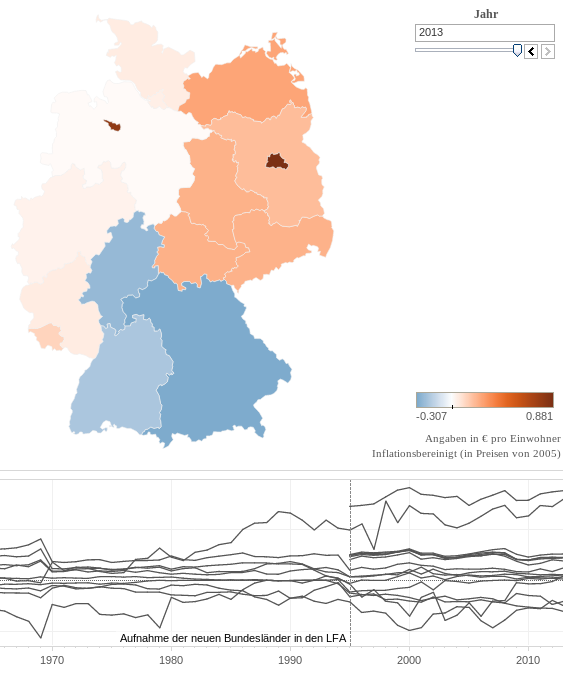
\includegraphics[scale=0.25]{section_open_data_politics.png}
  \end{figure}
  \column{0.5\textwidth}
  \begin{itemize}
   \item Politische Entscheidungen nachvollziehen und kontrollieren
   \item OK Lab Hamburg: Länderfinanzausgleich visualisieren \cite{Laefi}
  \end{itemize}
 \end{columns}
\end{frame}




\begin{frame}[t]{Warum Open Data?}
 \begin{columns}
  \column{0.4\textwidth}
  \begin{figure}[h]
   \centering
   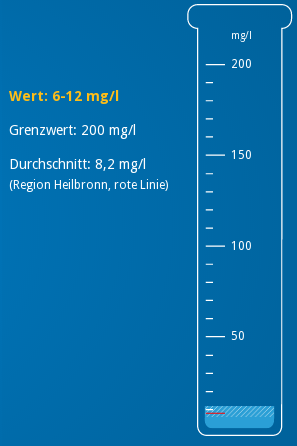
\includegraphics[scale=0.3]{section_open_data_complexity.png}
  \end{figure}
  \column{0.5\textwidth}
  \begin{itemize}
   \item Komplexe Sachverhalte besser verstehen
   \item OK Lab Heilbronn: Was steckt in meinem Leitungswasser \cite{Heilbronn}
  \end{itemize}
 \end{columns}
\end{frame}

\begin{frame}[t]{Warum Open Data?}
 \begin{columns}
  \column{0.4\textwidth}
  \begin{figure}[h]
   \centering
   
\includegraphics[scale=0.3]{section_open_data_innovation.png}
  \end{figure}
  \column{0.5\textwidth}
  \begin{itemize}
   \item Innovationen fördern
   \item Wheelmap \cite{Wheelmap}
   \item "Wheelmap.org ist eine Online-Karte zum Suchen, Finden und Markieren rollstuhlgerechter Orte."
  \end{itemize}
 \end{columns}
\end{frame}


